% Beginning code for all standard physics latex documents

%Created on: May 8, 2014    Edited by: Wesley Kyle
%Edited on:	May 12, 2016	Edited by: P. Gimby - cleaned up the code to remove unneeded packages
%Edited on:	May 13, 2016	Edited by: P. Gimby - collected a few more packages used in 325.
%Edited on:	May 16, 2016	Edited by: P. Gimby - fixed page numbering error.
%Edited on: May 20, 2016	Edited by: Alex Shook - Added packages for 497

\documentclass[justified]{tufte-book}
\usepackage{graphicx} % allow embedded images
\setkeys{Gin}{width=\linewidth,totalheight=\textheight,keepaspectratio}
\usepackage{amsmath}  % extended mathematics
\usepackage{bm}  % bold font in math mode
\usepackage{longtable} %lets long tables flow into multiple pages instead of running off the page or having to break tables up manually
\usepackage{booktabs} % book-quality tables
\usepackage{units}    % non-stacked fractions and better unit spacing
\usepackage{multicol} % multiple column layout facilities
\usepackage{tikz} %for drawing nice pictures
\usepackage{indentfirst} % makes first line of each new section be indented
\usepackage{enumitem} % extended options for the enumerate environment
\usepackage{soul} % gives more typestting options like spacing, underline, and strike-through
\usepackage{marvosym} %extra symbols package
\usepackage{multirow} % for special table controls
\usepackage[singlelinecheck=false]{caption} % allow captions w/o figure number
\captionsetup{compatibility=false} % corrects in issue with the caption package
\usepackage{float} % allows for contorl over position of figures and tables
\allowdisplaybreaks % allows equations to span two pages if needed
\usepackage{mathrsfs} % fancy math symbols
\usepackage{multirow} % for special table controls
\usetikzlibrary{arrows,shapes,snakes,calc,patterns,3d} % addon to tikz
\usetikzlibrary{circuits.ee.IEC} % addon to tikz
\usepackage{pgfplots} % package for making plots of functions
\usepackage{gensymb} % symbols i,e. degrees
\usetikzlibrary{decorations.pathmorphing} % to draw the springs
\tikzset{circuit declare symbol = ac source}
\tikzset{set ac source graphic = ac source IEC graphic}
\usepackage{changepage} % allows for full page environment
\usepackage{comment} % allows comment tags for large sections

% define new page style that puts page numbers in the middle
%\begin{comment}
\fancypagestyle{custom}{
\fancyhf{} % clear all header and footer fields
\fancyheadoffset{0pt}
\fancyfootoffset{0pt}
\fancyfoot[C]{\thepage}
\renewcommand{\headrulewidth}{0pt}
\renewcommand{\footrulewidth}{0pt}}
\pagestyle{custom}
%\end{comment}

%below creates a new circuit symbol for AC sources
\tikzset{
         ac source IEC graphic/.style=
          {
           transform shape,
           circuit symbol lines,
           circuit symbol size = width 3 height 3,
           shape=generic circle IEC,
           /pgf/generic circle IEC/before background=
            {
             \pgftransformresetnontranslations
             \pgfpathmoveto{\pgfpoint{-0.8\tikzcircuitssizeunit}{0\tikzcircuitssizeunit}}
             \pgfpathsine{\pgfpoint{0.4\tikzcircuitssizeunit}{0.4\tikzcircuitssizeunit}}
             \pgfpathcosine{\pgfpoint{0.4\tikzcircuitssizeunit}{-0.4\tikzcircuitssizeunit}}
             \pgfpathsine{\pgfpoint{0.4\tikzcircuitssizeunit}{-0.4\tikzcircuitssizeunit}}
             \pgfpathcosine{\pgfpoint{0.4\tikzcircuitssizeunit}{0.4\tikzcircuitssizeunit}}
             \pgfusepathqstroke
            }
          }
        }
% end of circuit symbol
%\begin{document}
%%%end individual beginning code/,$d


%  \begin{titlepage}
%    \vspace*{\fill}
%    \begin{center}
%      \huge{{\bf TITLE1}}\\[0.4cm]
%      \huge{TITLE2}\\[0.4cm]
%      \LARGE{Laboratory Manual}\\[0.4cm]
%      \large{SEASON YEAR}
%    \end{center}
%    \vspace*{\fill}
%  \end{titlepage}
%\maketitle

%\begin{spacing}{0.5}
%\tableofcontents
%\end{spacing}

%NEW PHYS 497 PACKAGES AND COMMANDS

%Subcaption package: Allows subfigures to be placed side by side, and labeled with individual captions (Added June 1, 2016)
\usepackage{subcaption}

%Array package: Allows for addiation specifications in arrays (Added May 6, 2016)
\usepackage{array}

%newcolumntype: Allows one to specify a fixed column width (Added May 6, 2016)
\newcolumntype{L}[1]{>{\raggedright\let\newline\\\arraybackslash\hspace{0pt}}m{#1}}
\newcolumntype{C}[1]{>{\centering\let\newline\\\arraybackslash\hspace{0pt}}m{#1}}
\newcolumntype{R}[1]{>{\raggedleft\let\newline\\\arraybackslash\hspace{0pt}}m{#1}}

%circuits.logic.US, circuits.logic.IEC: For drawing logic gates in Tikz (Added May 6, 2016) 
\usetikzlibrary{circuits.logic.US,circuits.logic.IEC}

\newcommand{\PGT}{ %PGT: positive going transition
\begin{tikzpicture}
\draw[-angle 60] (0,0) -- (0,5pt);
\draw (0,5pt) -- (0,6pt) -- (5pt,6pt);
\draw (-5pt,0) -- (0,0);
\end{tikzpicture}
}





%TEST
\usepackage{geometry}
\pagestyle{fancy}

%\usepackage[caption=false]{subfig}

%\makeatletter
%\renewenvironment{figure}[1][htbp]{%
%  \@tufte@orig@float{figure}[#1]%
%}{%
%  \@tufte@orig@endfloat
%}

%\renewenvironment{table}[1][htbp]{%
%  \@tufte@orig@float{table}[#1]%
%}{%
%  \@tufte@orig@endfloat
%}
%\makeatother

% use instead of subfigure
\makeatletter
\newenvironment{multifigure}[1][htbp]{%
  \@tufte@orig@float{figure}[#1]%
}{%
  \@tufte@orig@endfloat
}
\makeatother

\makeatletter
\newenvironment{mainfigure}[1][htbp]{%
\@tufte@orig@float{figure}[#1]
\begin{adjustwidth}{}{-153pt}}
{\end{adjustwidth}\@tufte@orig@endfloat}%
\makeatother

\makeatletter
\newenvironment{maintable}[1][htbp]{%
\@tufte@orig@float{table}[#1]
\begin{adjustwidth}{}{-153pt}}
{\end{adjustwidth}\@tufte@orig@endfloat}%
\makeatother

%%%% Labatorial Cross-over labs need this code. This should be temporary PG Dec 7, 2016

\newcounter{questioncounter}
\setcounter{questioncounter}{0}
\newcounter{checkpointcounter}
\setcounter{checkpointcounter}{0}
\newcounter{figurecounter}
\setcounter{figurecounter}{0}
%%%%%%%%%%%%%%%%%%%%%%%%%%%%%%%%%%%%%%%%%%%%%%%%%%%%%%%

\newcommand{\checkpoint}{
 \fbox{\begin{minipage}{0.2\textwidth}
 %\includegraphics[width=0.5\textwidth]{stop}
 \end{minipage}
 \begin{minipage}{1.0\textwidth}
 {\bf CHECKPOINT \addtocounter{checkpointcounter}{1} \arabic{checkpointcounter}: Before moving on to the next part, have your TA check the results you obtained so far.}
 \end{minipage}}}

%%% end labatorial cross-over code.

% New environment for placing figure captions under the figure
%\makeatletter
%\newenvironment{mainfigure}{\textwidth}[1][htbp]{%
%\@tufte@orig@float{figure}[#1]%
%}{%
%\@tufte@orig@endfloat
%}
%\makeatother

\begin{document}
%%%%%%%%%%%%%%%%%%%%%%%%%%%%%%%%%%%%%%%%%%%%%
%
% 0096 PHYS397FA2017
%
%%%%%%%%%%%%%%%%%%%%%%%%%%%%%%%%%%%%%%%%%%%%%


\setcounter{chapter}{5}
\setcounter{equation}{0}
\setcounter{table}{0}
\setcounter{figure}{0}
\chapter{Hall Effect and Magnetic Hysteresis}

\section{Equipment}

% first column
\begin{minipage}[t]{0.5\textwidth}
\begin{itemize}[noitemsep]
\item Electromagnet
\item Anatek power supply (2)
\item Fluke Multimeter (2)  %changed from 3 to 2
\item Philips PM2535 multimeter
\item InAs Hall probe
\item standard magnet
\item laboratory stand
\item fork clamp
\end{itemize}
\end{minipage}
%second column
\begin{minipage}[t]{0.5\textwidth}
\begin{itemize}[noitemsep]
\item right angle clamp
\item female BNC to male banana adaptor
\item BNC coaxial cable
\item set of connecting leads
\item compass
% \item plastic ruler - removed because not needed
\item calipers
\end{itemize}
\end{minipage}

\begin{marginfigure}[+2in]
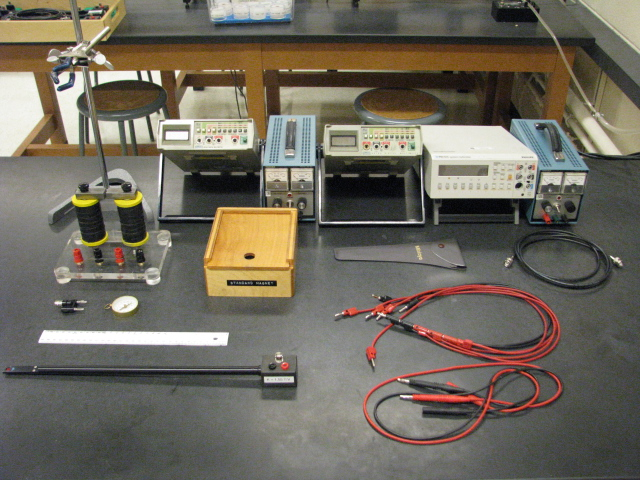
\includegraphics{/usr/local/master/labs/physics397-FA2017/0096-PHYS397FA2017/Hall-Effect-and-Magnetic-Hysteresis-Setup.jpg}
\caption{A photograph of the experimental setup.}
\label{fig:HEsetup}
\end{marginfigure}

\section{Preparation}
Review the fundamentals of the Hall effect. The derivation of the Hall voltage is provided in detail in the lab manual.

\section{Purpose}
To learn to calibrate a transducer, in this case a Hall probe, using known standards of magnetic field strength. To learn to identify hysteresis effects in physical systems. Lastly, be able to determine the density of charge carriers and drift velocity in a Hall probe.

\section{Theory}
Transducers are a general class of device that converts variations in a physical quantity into an electrical signal. One well studied example is a {\bf magnetic field transducer}, called a {\bf Hall probe}, which converts magnetic field intensity into potential differences. In this experiment the generation of Hall voltages through the Hall effect is examined. The Hall effect in an InAs semiconductor probe is explained in Section I. Hysteresis and the hysteresis curve of an iron core electromagnet, explained in section II,  are then examined using  a Hall probe. Lastly, the density of charge carriers and their drift velocity in a Hall probe are determined.

\section{I - The Hall Effect}
An investigation into the generation of potential differences across current carrying conductors immersed in a magnetic field, presently known as the {\bf Hall Effect} was initiated by Edwin Hall, then a graduate student, in 1879. The effect is thought to have escaped the attention of other researchers mainly because the potential differences were so small and difficult to measure.

Charges moving with drift velocity , in the presence of both a magnetic field, $\vec{B}$, and an electric field, $\vec{E}$, experience a total force known as the Lorentz force, $\vec{F}$, given by 

\begin{equation}
\vec{F}=\vec{F}_E+\vec{F}_M=q\cdot \vec{E}+q\cdot \vec{\nu}\times \vec{B}
\label{equ:he1}
\end{equation}

\noindent where $F_E$ and $F_M$ are the electric and magnetic force vectors respectively and q is the elementary electronic charge. Since charge carriers in a conductor undergo random motion similar to the motion of molecules in a gas, the drift velocity, $\vec{\nu}$, is an average velocity of the charge carriers.

\begin{figure}
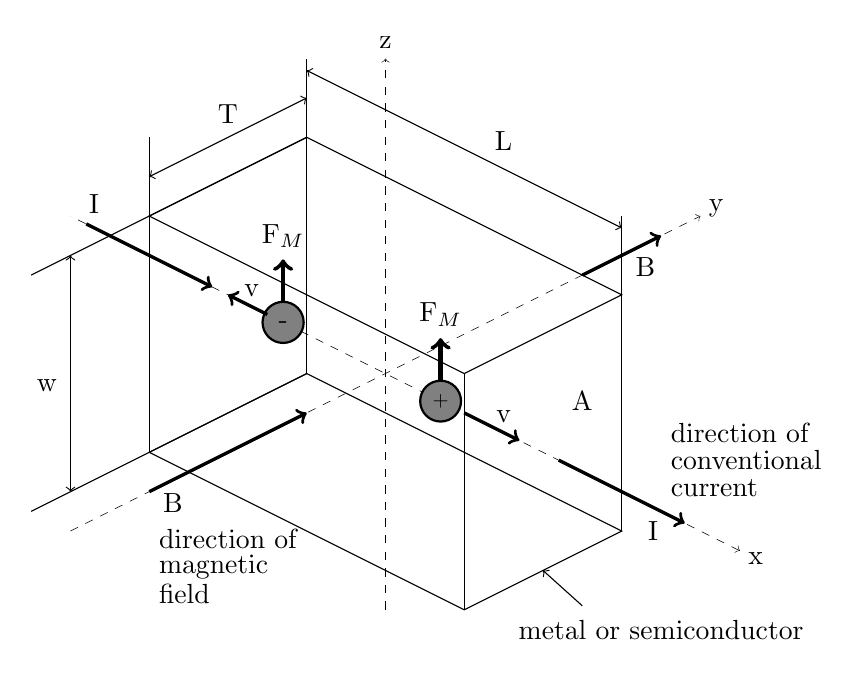
\begin{tikzpicture}[y={(-1cm,0.5cm)},x={(1cm,.5cm)}, z={(0cm,1cm)}]
% coordinate system
\coordinate (O) at (0, 0, 0);
\draw[very thin,dashed,->](-4,0,0)--(4,0,0);
\draw[very thin,dashed,<-](0,-4.5,0)--(0,4,0);
\draw[very thin,dashed,->](0,0,-3)--(0,0,4);
%volume element
\node [shape=circle,draw=black,thick,fill=gray,scale=1] at (0,1.3,0){-};
\node [shape=circle,draw=black,thick,fill=gray,scale=.75] at (0,-.7,0){+};
%indicator lines
\draw[ultra thick,->](0,1.3,.25)--(0,1.3,.8);
\draw[ultra thick,->](0,-.7,.25)--(0,-.7,.8);
\draw (-1,-2,-1.5)--(-1,2,-1.5)--(1,2,-1.5)--(1,-2,-1.5)--cycle;
\draw (-1,-2,1.5) -- (-1,2,1.5) -- (1,2,1.5) -- (1,-2,1.5) -- cycle;
\draw[thin](1,2,-1.5)--(-2.5,2,-1.5);
\draw[thin](1,2,1.5)--(-2.5,2,1.5);
\draw[thin,<->](1,2,2)--(-1,2,2); %T
\draw[thin,<->](-2,2,-1.5)--(-2,2,1.5); %W
\draw[thin,<->](1.5,-1.5,1.85)--(1.5,2.5,1.85); %L
\draw(-1,-2,-1.5)--(-1,-2,1.5);
\draw(-1,2,-1.5)--(-1,2,1.5);
\draw[thin](-1,2,-1.5)--(-1,2,2.5);
\draw(1,2,-1.5)--(1,2,1.5);
\draw[thin](1,2,-1.5)--(1,2,2.5);
\draw(1,-2,-1.5)--(1,-2,1.5);
\draw[thin](1,-2,-1.5)--(1,-2,2.5);
\node at (0,0,4.2){z};
\node at (4.2,0,0){y};
\node at (0,-4.7,0){x};
\node at (-3,-.3,0){B};
\node at (3,-.3,0){B};
\node at (0,3.7,.3){I};
\node at (0,-3.4,-.3){I};
\node at (0,-.7,1.1){F$_M$};
\node at (0,1.3,1.1){F$_M$};
\node at (0,-1.5,.2){v};
\node at (0,1.7,.2){v};
\node at (0,-2.5,.9){A};
\node at (-2.3,2,0){w};
\node at (0,2,2.3){T};
\node at (1.5,0,2.2){L};
\node[right] at (-3,0,-.6){direction of};
\node[right] at (-3,0,-.95){magnetic};
\node[right] at (-3,0,-1.3){field};
\node[right] at (-0,-3.5,1){direction of};
\node[right] at (-0,-3.5,.65){conventional};
\node[right] at (0,-3.5,.3){current};
\node at (1.5,-2,-3){metal or semiconductor};
\draw[->,thin](-1.7,-4.2,0)--(-1.5,-3.5,0);
\draw[very thick,->](-3,0,0)--(-1,0,0); %B
\draw[very thick,->](2.5,0,0)--(3.5,0,0); %B
\draw[very thick,->](0,-1,0)--(0,-1.7,0); %v
\draw[very thick,->](0,1.5,0)--(0,2,0); %v
\draw[very thick,->](0,3.8,0)--(0,2.2,0); % I
\draw[very thick,->](0,-2.2,0)--(0,-3.8,0); % I
\end{tikzpicture}
\caption{Current flow through a volume element of a metal or semiconductor.}
\label{fig:he1}
\end{figure}

	As illustrated in Figure \ref{fig:he1}, current can be viewed either as a flow of positive charges in one direction or as a flow of negative charges in the opposite direction. If the polarity of the majority charge carriers is negative, the current will be due to the flow of electrons; otherwise it will be due to the flow of holes (positive charges). The direction of flow for positive charges is referred to as the direction of conventional current.
	Charges deflected by the action of the magnetic field, accumulate at the edges of the conductor and a transverse electric field, $\vec{E}$, appears across the conductor. The process of charge deflection and separation continues until the magnitudes of $\vec{F}_E$ and $\vec{F}_M$ have become equal and charges can no longer be deflected against the induced electric field. An equilibrium is established where the total Lorentz force, $\vec{F}$, is equal to zero and a small potential difference, called the {\bf Hall voltage}, appears across the conductor. The polarity of the Hall voltage is determined by the polarity of the charge carriers alone because, as can be seen from Figure \ref{fig:he1}, the magnetic force on a charge carrier of either polarity is always in the same direction. The polarity of the Hall voltage is thus a function of the polarity of the majority charge carriers for that conductor. 
	Another important factor is the relative abundance of carriers of either polarity. In a hypothetical situation, such as the one shown in Figure \ref{fig:he1}, where the ratio of the positive to negative carriers is one to one, the Hall voltage would vanish because of cancellation. Predominance of one type of current carrier, negative or positive is thus essential. The effect could not occur in semiconductors where both types of carriers appear in equal concentrations.
	Prior to Hall's work, conduction in metals was thought to have been caused entirely by a flow of negative charges (electrons). Experiments with various metals have shown, however, that this was not always true. It was discovered that current, in some metals, could be carried by positive charges (holes) not electrons. The phenomenon remained unexplained at the time and came to be known as the {\bf Anomalous Hall Effect}. 
	Semiconductors, unknown at the time of Hall's investigation, exhibit properties similar to those of metals. Here however, the current densities are lower and the Hall voltages are higher than in metals. Since higher voltages are easier to measure, semiconductor Hall probes are routinely used for the measurement of magnetic fields. 
	The information required to find an expression for the Hall voltage is given in Equation \ref{equ:he1}. Since $\vec{F}=0$ at equilibrium, it is true that

\begin{equation}
q\nu B=qE
\label{equ:he2}
\end{equation}

\noindent so

\begin{equation}
\nu B=E
\label{equ:he3}
\end{equation}

\noindent The {\bf Hall voltage}, $V_H$, is then

\begin{equation}
V_H=Ew=\nu Bw
\label{equ:he4}
\end{equation}

\noindent since the potential difference, $V_H$, appearing across the conductor of width $w$, is given by the product of the electric field magnitude and the width of the conductor. Equation \ref{equ:he4} can then be rearranged to read

\begin{equation}
B=KV_H
\label{equ:he5}
\end{equation}

\noindent where K, a proportionality constant, is equal to $1/\nu w$. Equation \ref{equ:he5} illustrates how the Hall voltage can be used in a transducer for the measurement of magnetic fields. If a semiconductor is placed in a magnetic field, then the Hall voltage developed across it can be measured directly with a volmeter. The magnetic field, B, is then found from Equation \ref{equ:he5}. Moreover, since Equation \ref{equ:he5} is linear, once the proportionality constant K is known,  any magnetic field can be determined. The procedure used to find K for a particular transducer is to subject the transducer to a known magnetic field and measure the Hall voltage. The proportionality constant for that transducer then is B/V$_H$. This procedure of {\bf calibrating the transducer} must always be performed before a transducer can be used for making measurements.

Charge carrier density, $n$, defined as the number of charge carriers per unit volume, can be determined from the measurement of the current in a conductor, as current is related to the motion of charged particles. As a rule, charge densities tend to be higher in metals than in semiconductors.

For a volume element , like the one shown in Figure \ref{fig:he2}, it is true that

\begin{equation}
\Delta V=A\Delta x
\label{equ:he6}
\end{equation}

\begin{marginfigure}
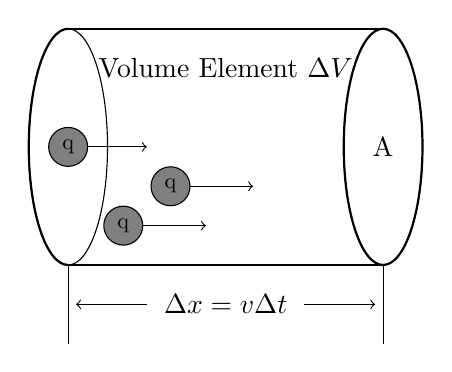
\begin{tikzpicture}
\draw(-2,0) ellipse (.5 and 1.5);
\draw[thick](2,0) ellipse (.5 and 1.5);
\draw[thick](-2,1.5)--(2,1.5);
\draw[thick](-2,-1.5)--(2,-1.5);
\node[black,draw=black,fill=gray,shape=circle,scale=.8] at (-1.3,-1){q};
\node[black,draw=black,fill=gray,shape=circle,scale=.8] at (-2,0){q};
\node[black,draw=black,fill=gray,shape=circle,scale=.8] at (-.7,-.5){q};
\node at (0,1){Volume Element $\Delta V$};
\node at (2,0){A};
\node at (0,-2){$\Delta x=v\Delta t$};
\draw[->](-1,-2)--(-1.9,-2);
\draw[->](1,-2)--(1.9,-2);
\draw(-2,-1.5)--(-2,-2.5);
\draw(2,-1.5)--(2,-2.5);
\draw[->](-1.05,-1)--(-.25,-1);
\draw[->](-1.75,0)--(-1,0);
\draw[->](-.45,-.5)--(.35,-.5);
\draw[thick](-2,1.5) arc (90:270:.5 and 1.5);
\end{tikzpicture}
\caption{Charge flow through a volume element.}
\label{fig:he2}
\end{marginfigure}

So if the charge carrier density is constant,then $\Delta V$ contains $nA\Delta x$ charge carriers. A {\bf charge element}, $\Delta Q$, contained in the volume element, $\Delta V$, is then given by

\begin{equation}
\Delta Q=nqA\Delta x
\label{equ:he7}
\end{equation}

\noindent where q is the elementary electronic charge, $1.602\times10^{-19}$ C.

For charges moving with drift velocity $\vec{\nu}$, $\Delta x$ is the distance covered in a time interval $\Delta t$. Thus

\begin{equation}
\Delta x=\nu \Delta t
\label{equ:he8}
\end{equation}

\noindent The charge element $\Delta Q$ can now be written as

\begin{equation}
\Delta Q=nqA\nu \Delta t
\label{equ:he9}
\end{equation}

\noindent Dividing both sides of Equation \ref{equ:he9} by $\Delta t$ yields

\begin{equation}
\dfrac{\Delta Q}{\Delta t}=I=nqA\nu
\label{equ:he10}
\end{equation}

\noindent where $I$ is the current flowing through the area $A$. Solving Equation \ref{equ:he10} for drift velocity $\nu$ gives

\begin{equation}
\nu=\dfrac{I}{nqA}
\label{equ:he11}
\end{equation}

\noindent Substituting an expression for the drift velocity $\nu$ from Equation \ref{equ:he4} gives

\begin{equation}
V_H=\dfrac{IBw}{nqA}
\label{equ:he12}
\end{equation}

\noindent As can be seen from Figure \ref{fig:he1}, $A$, the cross sectional area of the conductor, is equal to the product of its width, $w$, and thickness, $T$. Equation \ref{equ:he12} can thus be simplified to

\begin{equation}
V_H=\dfrac{IB}{nqT}
\label{equ:he13}
\end{equation} 

\noindent The quantity $1/nq$ is known as the {\bf Hall coefficient}, $R_H$. When the semiconductor is used as a probe to measure magnetic fields, it is excited with a constant current called the {\bf control current}, $I_c$. So $I$ is renamed to $I_c$ and Equation \ref{equ:he13} becomes

\begin{equation}
V_H=R_H\dfrac{I_c}{T}B
\label{equ:he14}
\end{equation}

The sensor element of the Hall probe is made of indium-arsenide. To measure magnetic flux density, the probe is first energized by allowing a steady control current to flow through it. Figure \ref{fig:he3} shows how the Hall sensor probe is connected for the measurements of magnetic fields. The probe is then immersed in a magnetic field such that its direction is perpendicular to the plane of the sensor element. 

\begin{figure}
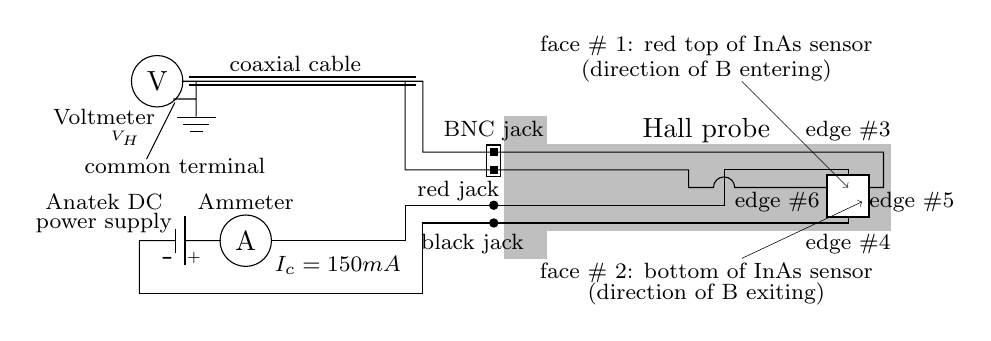
\begin{tikzpicture}[circuit ee IEC,scale=.9,inner sep=3pt]
\draw[black,fill=lightgray,draw=lightgray](5.15,.5)rectangle(5.75,2.5); %grey for probe
\draw[black,fill=lightgray,draw=lightgray](5.15,.9)rectangle(10.6,2.1); %grey for probe
\draw(0,0)--(4,0)--(4,1)--(10,1)--(10,1.75)--(8.25,1.75)--(8.25,1.25)--(3.75,1.25)
--(3.75,.75)--(1.5,.75)node[black,shape=circle,draw=black,fill=white]{A};
\draw(1.15,.75) to [battery](0,.75)--(0,0); %bottom circuit
\node[black,fill=white,draw=black,shape=circle,scale=1] at (.25,3){V}; %voltmeter
\draw[double distance=2,thick](3.9,3)--(.7,3); %coaxial
\draw(.6,3)--(3.75,3)--(3.75,1.75)--(7.75,1.75)--(7.75,1.5)--(8.1,1.5) arc (180:0:.15)
--(10.5,1.5)--(10.5,2)--(4,2)--(4,3)--(4,3)--(.8,3)--(.8,2.5)--(.8,2.75)--(.48,2.75); %top circuit
\draw(.8,2.5) to[ground](.8,2.28); %ground
\node[black,fill=black,shape=circle,scale=.4] at(5,1){}; %black jack
\node[black,fill=black,shape=circle,scale=.4] at(5,1.25){}; %red jack
\draw(4.9,1.65)rectangle(5.1,2.1); %BNC jack
\node[black,fill=black,shape=rectangle,scale=.5] at(5,2){}; %BNC jack
\node[black,fill=black,shape=rectangle,scale=.5] at(5,1.75){}; %BNC jack
\node[black,thick,fill=white,draw=black,shape=rectangle,scale=2.5] at(10,1.38){}; %InAs sensor

%labels
\node[font=\tiny] at (.77,.5){+};
\node[font=\large] at (.4,.5){-};
\node[font=\footnotesize] at (-.5,2.5){Voltmeter};
\node[font=\tiny] at (-.2,2.2){$V_H$};
\node[font=\footnotesize] at (.5,1.8){common terminal};
\draw[thin](.1,1.9)--(.5,2.7);
\node[font=\footnotesize] at (1.5,1.3){Ammeter};
\node[font=\footnotesize] at (-.5,1.3){Anatek DC};
\node[font=\footnotesize] at (-.5,1){power supply};
\node[font=\footnotesize] at (2.2,3.25){coaxial cable};
\node[font=\footnotesize] at (5,2.3){BNC jack};
\node[font=\footnotesize] at (4.5,1.45){red jack};
\node[font=\footnotesize] at (4.7,.7){black jack};
\node[font=\normalsize] at (8,2.3){Hall probe};
\node[font=\footnotesize] at (10,2.3){edge \#3};
\node[font=\footnotesize] at (10,.7){edge \#4};
\node[font=\footnotesize] at (10.9,1.3){edge \#5};
\node[font=\footnotesize] at (9,1.3){edge \#6};
\node[font=\footnotesize] at (8,3.5){face \# 1: red top of InAs sensor};
\node[font=\footnotesize] at (8,3.15){(direction of B entering)};
\draw[very thin,->](8.5,3)--(10,1.5);
\node[font=\footnotesize] at (8,.3){face \# 2: bottom of InAs sensor};
\node[font=\footnotesize] at (8,0){(direction of B exiting)};
\draw[very thin,->](8.5,.5)--(10.2,1.3);
\node[font=\footnotesize] at (2.8,.4){$I_c=150mA$};

\end{tikzpicture}
\caption{Schematic of the Hall probe sensor setup.}
\label{fig:he3}
\end{figure}

The Hall voltage that develops across the probe is small, of the order of a few millivolts, so it is good practice to shield it from sources of external noise, which is why a coaxial cable is used. The polarity of the Hall voltage depends on the type of charge carrier active in the semiconductor and can be determined from the polarity of the observed Hall voltage. The polarities of the electrical connections shown in Figure \ref{fig:he3} are in agreement with the sign conventions introduced earlier in Figure \ref{fig:he1}.

The mounting of the semiconductor wafer inside the Hall probe makes it impractical to measure its dimensions directly. For the purposes of this experiment the following dimensions, given by the manufacturer, can be used in the calculations. The thickness of the semiconductor wafer, T, is equal to $(8\pm 1)\times10^{-5}$m. The width of the Hall plate, w, is equal to $(2.03\pm0.01)\times10^{-3}$m. Its length, L, is equal to $(4.57\pm0.01)\times10^{-3}$m.

\section{Magnetic Hysteresis}

All matter is made up of atoms that contain moving electrons. Associated with every atom, there is a tiny {\bf magnetic moment} that is partly due to the orbital motion of the atomic electrons and partly due to their spin. In some materials the magnetic moments remain at random and the substance appears non-magnetic. In others, large numbers of magnetic moments are oriented in some sense or the presence of an external magnetic field causes them to orient in some sense. When this happens, the material becomes {\bf magnetized} and begins to generate its own magnetic field. 

\begin{marginfigure}
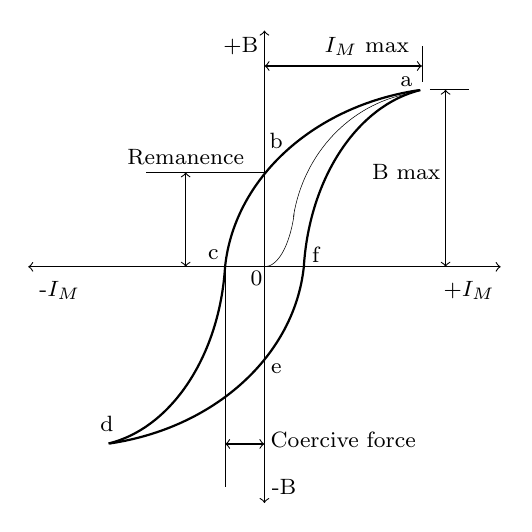
\begin{tikzpicture}
%axes
\draw[<->](-3,0)--(3,0);
\draw[<->](0,-3)--(0,3);
%this is the SWOOSH
\draw[thick](-.5,0) arc (175:100:3 and 2.5);
\draw[thick](.5,0) arc (-5:-80:3 and 2.5);
\draw[thick](.5,0) arc (175:100:1.8 and 2.5);
\draw[thick](-.5,0) arc (-5:-80:1.8 and 2.5);
\draw[very thin](0,0) arc (-90:-20:.4 and 1)--(.37,.65) arc (170:100:1.8 and 1.91);
%demarcation lines
\draw[very thin](0,1.2)--(-1.5,1.2);
\draw[very thin](2,2.35)--(2,2.8);
\draw[very thin](2.1,2.25)--(2.6,2.25);
\draw[very thin](-.5,0)--(-.5,-2.8);
\draw[<->](-1,0)--(-1,1.2);
\draw[<->](2.3,0)--(2.3,2.25);
\draw[<->](0,2.55)--(2,2.55);
\draw[<->](-.5,-2.25)--(0,-2.25);
%labels
\node[font=\footnotesize] at(-1,1.4){Remanence};
\node[font=\footnotesize] at(1.3,2.8){$I_M$ max};
\node[font=\footnotesize] at(1.8,1.2){B max};
\node[font=\footnotesize] at(1,-2.2){Coercive force};
\node[font=\footnotesize] at(.25,-2.8){-B};
\node[font=\footnotesize] at(-.3,2.8){+B};
\node[font=\footnotesize] at(-2.6,-.3){-$I_M$};
\node[font=\footnotesize] at(2.6,-.3){+$I_M$};
\node[font=\footnotesize] at(1.8,2.35){a};
\node[font=\footnotesize] at(.15,1.6){b};
\node[font=\footnotesize] at(-.65,.15){c};
\node[font=\footnotesize] at(-2,-2){d};
\node[font=\footnotesize] at(.15,-1.3){e};
\node[font=\footnotesize] at(.65,.15){f};
\node[font=\footnotesize] at(-.1,-.15){0};
\end{tikzpicture}
\caption{Hysteresis in a magnetized ferromagnetic material.}
\label{fig:he4}
\end{marginfigure}

In ferromagnetic materials, strong interaction between atomic magnetic moments leads to an alignment of these moments in regions called {\bf magnetic domains}, consisting of a large number of magnetic moments. The alignment within the magnetic domains exists even in the absence of an external magnetic field, but the domains are pointed randomly. When an external magnetic field is applied however, the domains tend to orient themselves parallel to the external field, producing a strong net magnetization effect. As the external field intensity is increased, more and more magnetic domains are aligned with the external field increasing the magnetization of the material. At some point virtually all magnetic domains are aligned and the sample reaches a state of {\bf magnetic saturation}. 

If a de-magnetizing field (magnetizing field of opposite polarity) is now applied to the sample, the de-magnetization of the sample lags behind the applied de-magnetizing field. This property, whereby the magnetic flux through the substance does not depend solely on the external magnetic field but also on the magnetic history, is referred to as the {\bf magnetic hysteresis}. When such a substance is subjected to periodic changes in magnetization, the energy dissipated through the production of heat due to the realignment of the magnetic domains, is known as the magnetic hysteresis loss. 

As indicated in Figure \ref{fig:he4}, initial magnetization of a ferromagnetic material corresponds to segment 0-a on the curve. At point a, which corresponds to a maximum on the curve, the material reaches a state of positive magnetic saturation. At this point, all magnetic domains are aligned in the positive direction and increases in the intensity of the magnetizing current have no further effect on the degree of magnetization. Now, as the intensity of the magnetizing current decreases towards zero, the magnetic flux density does not decrease along path a-0. Instead, it decreases along path a-b. This is because some magnetic domains remain aligned and the material retains some degree of magnetization even in the absence of a magnetizing current. The property whereby ferromagnetic materials retain some of their flux density, is referred to as {\bf remanence} or {\bf residual magnetism}. To reduce the remanence to zero, a reverse magnetizing force must be applied. This is accomplished by reversing the magnetizing current (the reverse magnetizing current is sometimes called the de-magnetizing current) and increasing its intensity. With an increase in the reverse current, the flux density drops off to zero along path b-c. The de-magnetizing force required to accomplish this task is called the {\bf coercive force}. As the de-magnetizing force increases beyond point c, the flux density begins to increase in the negative direction, completing segment c-d on the curve. At point d, which represents the minimum on the curve, negative magnetic saturation is reached and all magnetic domains are aligned in the opposite direction. At this point, further increases in the intensity of the de-magnetizing current have no effect on the state of magnetization. The return leg of the magnetization (re-magnetization) process, between points d-e-f-a, is just the reverse of the process described above. It is completed by first decreasing the de-magnetizing force to zero between points d-e, then increasing the magnetizing force in the positive direction between points e-a. The process is complete when the sample returns to its state of positive saturation at point a.

The magnetic field to be measured is generated in an {\bf electromagnet}. Figure \ref{fig:he5} is the the circuit diagram for the electromagnet, power supply, and ammeter. Direct current passing through the coils magnetizes the iron core of the electromagnet and the resultant magnetic flux density is measured in the air gap (see Figures \ref{fig:he5} and \ref{fig:he6}). Since iron is ferromagnetic the characteristics of the magnetic field produced in it are determined by a magnetic hysteresis curve similar to the one shown in Figure \ref{fig:he4}.

\section{Experimental Procedure}
\begin{enumerate}

\item Fasten the Hall probe to the lab stand with the extension clamp. Connect the power supply to the control current inputs on the body of the Hall probe, as shown in Figure \ref{fig:he3}. Insert a dual banana plug across the voltage and common terminals of the multimeter. The small rectangular tab on the body of the dual plug indicates ground or common polarity. Make the Hall voltage connection from the coaxial jack on the probe to the multimeter using a coaxial cable. Using a single connecting lead, connect the common terminal of the multimeter to the green grounding terminal of the power supply. This connection is necessary to ensure that the lower contact on the InAs probe is at ground potential while the control current potentials are floating. Do not ground either the positive or the negative terminal of the Anatek power supply as this would place one end of the Hall probe at the same ground potential as the negative end of the probe. As a result, the equipotential lines across the sensor would be skewed, producing a Hall voltage even in the absence of a magnetic field. 

\begin{marginfigure}
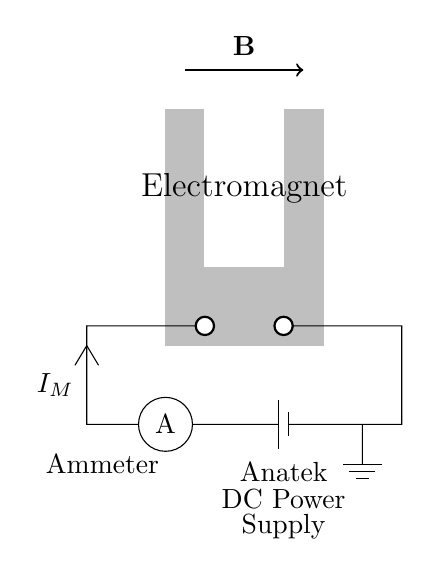
\begin{tikzpicture}[circuit ee IEC]
%electromagnet
\draw[fill=lightgray,draw=lightgray](2,3)rectangle(4,6);
\draw[fill=white,draw=white](2.5,4)rectangle(3.5,6.1);
%circuit
\draw[](2.5,3.25)--(1,3.25)--(1,2)--(2,2)node[fill=white,draw=black,shape=circle,scale=1]{A}
to [battery](5,2)--(5,3.25)--(3.5,3.25);
\draw(4.5,2) to [ground={pos=1}](4.5,1.4);
\node[fill=white,draw=black,shape=circle,thick,scale=.7] at (2.5,3.25){};
\node[fill=white,draw=black,shape=circle,thick,scale=.7] at (3.5,3.25){};
%labels
\node at(3,6.8){{\bf B}};
\draw[->,thick](2.25,6.5)--(3.75,6.5);
\node[font=\large] at(3,5){Electromagnet};
\node at(1.2,1.5){Ammeter};
\node at(3.5,1.4){Anatek};
\node at(3.5,1.05){DC Power};
\node at(3.5,.7){Supply};
\node at(.6,2.5){$I_M$};
\draw(.85,2.75)--(1,3)--(1.15,2.75);
\end{tikzpicture}
\caption{Circuit diagram for electromagnet power supply.}
\label{fig:he5}
\end{marginfigure}

\begin{marginfigure}[+25mm]
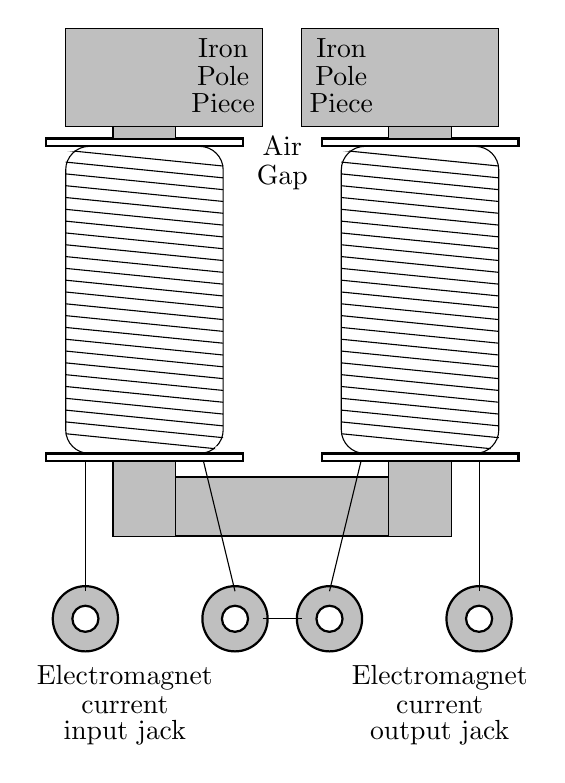
\begin{tikzpicture}
%solenoids
\draw[rounded corners=3mm](.25,.1)--(.25,4)--(2.25,4)--(2.25,.1)--cycle;
\draw[rounded corners=3mm](3.75,.1)--(3.75,4)--(5.75,4)--(5.75,.1)--cycle;
\foreach \y in {0,...,24}
{
\draw(.25,.35+\y*.15)--(2.25,.15+\y*.15);
\draw(3.75,.35+\y*.15)--(5.75,.15+\y*.15);
}
\draw[thick](0,0)rectangle(2.5,.1);
\draw[thick](0,4)rectangle(2.5,4.1);
\draw[thick](3.5,0)rectangle(6,.1);
\draw[thick](3.5,4)rectangle(6,4.1);
%iron pole pieces
\draw[fill=lightgray](.25,4.25)rectangle(2.75,5.5);
\draw[fill=lightgray](.85,4.1)rectangle(1.65,4.25);
\draw[fill=lightgray](3.25,4.25)rectangle(5.75,5.5);
\draw[fill=lightgray](4.35,4.1)rectangle(5.15,4.25);
%base
\draw[thick,fill=lightgray](1.64,-.95)rectangle(4.36,-.2);
\draw[fill=lightgray](.85,0)rectangle(1.65,-.95);
\draw[fill=lightgray](4.35,0)rectangle(5.15,-.95);
%jacks
\node[draw=black,thick,fill=lightgray,shape=circle,scale=2.5] at (.5,-2){};
\node[draw=black,thick,fill=lightgray,shape=circle,scale=2.5] at (2.4,-2){};
\node[draw=black,thick,fill=lightgray,shape=circle,scale=2.5] at (3.6,-2){};
\node[draw=black,thick,fill=lightgray,shape=circle,scale=2.5] at (5.5,-2){};
\node[draw=black,thick,fill=white,shape=circle,scale=1] at (.5,-2){};
\node[draw=black,thick,fill=white,shape=circle,scale=1] at (2.4,-2){};
\node[draw=black,thick,fill=white,shape=circle,scale=1] at (3.6,-2){};
\node[draw=black,thick,fill=white,shape=circle,scale=1] at (5.5,-2){};
%labels and such
\node[]at(2.25,5.25){Iron};
\node[]at(3.75,5.25){Iron};
\node[]at(2.25,4.9){Pole};
\node[]at(3.75,4.9){Pole};
\node[]at(2.25,4.55){Piece};
\node[]at(3.75,4.55){Piece};
\node[]at(3,4){Air};
\node[]at(3,3.6){Gap};
\node[]at(1,-2.75){Electromagnet};
\node[]at(1,-3.1){current};
\node[]at(1,-3.45){input jack};
\node[]at(5,-2.75){Electromagnet};
\node[]at(5,-3.1){current};
\node[]at(5,-3.45){output jack};
\draw(.5,-1.65)--(.5,0);
\draw(5.5,-1.65)--(5.5,0);
\draw(2.4,-1.65)--(2,0);
\draw(3.6,-1.65)--(4,0);
\draw(2.75,-2)--(3.25,-2);
%white space
\draw[white,very thick](2.3,.15)--(2.15,.17);
\draw[white,very thick](.2,3.96)--(.35,3.96);
\draw[white,very thick](3.7,3.96)--(3.85,3.96);
\draw[white,very thick](5.65,.15)--(5.9,.17);
\end{tikzpicture}
\caption{Diagram of the electromagnet.}
\label{fig:he6}
\end{marginfigure}

\item Have your lab instructor check your circuit before turning on any of the power supplies. Insert the Hall probe into the standard magnet (the magnitude of B$_{cal}$ is stated on the magnet), center it in the gap, and at a constant control current of 150 mA, measure its Hall voltage output to find constant K from Equation \ref{equ:he5}. This calibrates the Hall probe so it can be used to measure other magnetic fields.

\item When K has been determined, set the air gap of the electromagnet to approximately 3.5 mm (see Figure \ref{fig:he6}). Place the Hall probe in the gap and take a series of Hall voltage versus electromagnet current readings (in steps of 0.1 A). Because of the residual magnetism in the core, take the readings for the full range of electromagnet currents in both directions. This means starting from $I=0$ (Figure \ref{fig:he4}), increasing the current to $I=+I_M$, decreasing back to $I=0$, reversing the electromagnet polarity and increasing to $I=-I_M$, decreasing back to $I=0$, reversing the polarity on the electromagnet again, and increasing back to $I=+I_M$. To get stable Hall voltage readings, the electromagnet current should be adjusted gradually, in one direction only.

\item Using the calibrated Hall probe as your measuring instrument, set the magnetic intensity of the electromagnet to 0.2 T. It is necessary to use the same probe control current that was used for probe calibration. Keeping the magnetic field constant at 0.2 T, record a series of Hall voltage versus control current readings over a range of 0 to 150 mA.

\item Make a sketch of the Hall probe, magnetic field and control current orientations with respect to the coordinate axes. Use a compass to determine the direction of magnetic field if necessary. Using the information from Figures \ref{fig:he1} and \ref{fig:he3} and the polarity of the Hall voltage output, find which type of majority charge carrier is responsible for the conduction of current through the probe.

\end{enumerate}

\section{Error Analysis}

A significant source of systematic error lies in the instability of the Hall voltage readings due to the heating of the Hall probe and the electromagnet. Other sources of error may be found in the non-uniformity of the magnetic fields produced in both the electromagnet and calibration magnet air gaps. Further errors may be introduced by non-uniform positioning of the probe in the calibration magnet gap or the tilting of the probe in the electromagnet gap while taking measurements. Such experimental inconsistencies would lead to a measurement of a component of the magnetic flux density instead of the entire flux density. Lastly, there is an error associated with the exact value of the magnetic flux density of the calibration magnet. The experimental uncertainties in I and B are determined from the uncertainties of the measuring instruments and can be readily estimated. The uncertainty in K can be determined from the uncertainties associated with the Hall voltage and the calibration magnetic flux density readings. 

\begin{marginfigure}
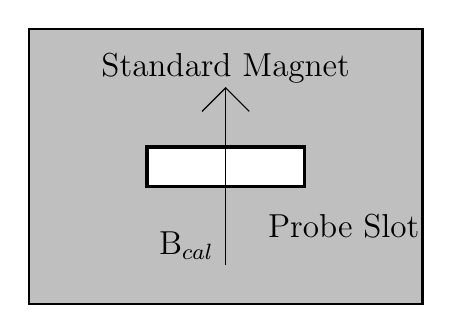
\begin{tikzpicture}
\draw[thick,fill=lightgray](0,0)rectangle(5,3.5);
\draw[very thick,fill=white](1.5,1.5)rectangle(3.5,2);
\draw[](2.5,.5)--(2.5,2.75);
\draw[](2.2,2.45)--(2.5,2.75)--(2.8,2.45);
\node[font=\large]at(2.5,3){Standard Magnet};
\node[font=\large]at(2,.75){B$_{cal}$};
\node[font=\large]at(4,1){Probe Slot};
\end{tikzpicture}
\caption{Standard magnet.}
\label{fig:he7}
\end{marginfigure}

\section{To be handed in to your lab instructor}

%%% begin prelab %%%
\section{Prelab}
\begin{enumerate}

\item Provide clear and concise definitions for the following terms related to this experiment: transducer, Hall voltage, drift velocity, charge carrier density, hole, magnetic moment, hysteresis.

\item Provide several examples of physical processes that exhibit hysteresis.

\item A Hall probe of thickness 100 microns is being used at a current of 50 mA.  The semiconductor in the probe is doped to a carrier density of $7.5\times10^{20}$ m$^{-3}$.  If the Hall voltage is measure to be 7 mV, what is the magnetic field strength?
\end{enumerate}
%%% end prelab %%%

\section{{\bf Data Requirements}}
\begin{enumerate}[resume]

\item The magnitude of the Hall voltage for the standard magnet.  From this, the numerical value of the proportionality constant, K, with error, can be determined using from Equation \ref{equ:he5} (procedure step 2).

\item A data table of Hall voltage versus electromagnet current at a constant probe control current of 150 mA (procedure step 3).

\item A data table of Hall voltage versus control current (procedure step 4). 

\item A sketch of your complete Hall probe experimental system as described in procedure step 5.  What is the sign of the charge carriers in this Hall probe.

\section{Calculations}
\item Using the experimental value of K, calculate the numerical value of the drift velocity, $\nu$, with error.

\item Calculate the magnetic flux density for each electromagnet current at a constant probe control current of 150 mA from your results in data requirement 5.
 
\item Produce a graph of magnetic intensity versus electromagnetic current.

\item Produce a graph of the Hall voltage versus control current.

\item Calculate the numerical value of the Hall coefficient, $R_H$, with error. 

\item Calculate the numerical value of the charge carrier density, $n$, with error, for Indium Arsenide.

\section{Discussion}

\item What does the graph of magnetic intensity versus electromagnetic current represent? Discuss the appearance of the plot you generate in Calculation part 11. Is this how you would expect an electromagnet to behave?

\item What is the remanence of the electromagnet? 

\item Discuss the impact of magnetic hysteresis on the use of electromagnets.

\item What are the two main sources of heat responsible for warming the Hall probe? 

\item What possible applications are there for the use of Hall probes and electromagnets.

\end{enumerate}


\AtEndDocument{\clearpage\ifodd\value{page}\else\null\clearpage\fi} % forces even page count, for double siding

%%%%%%%%%%%%%%%%%%%%%%%%%%%%%%%%%%%%%%%%%%%%%
%
% 0096 PHYS397FA2017 - Companion Guide
%
%%%%%%%%%%%%%%%%%%%%%%%%%%%%%%%%%%%%%%%%%%%%%


\chapter{The Hall Effect and Magnetic Hysteresis - Companion Guide}

\section{Equipment}
% first column
\begin{minipage}[t]{0.5\textwidth}
\begin{itemize}[noitemsep]
\item Electromagnet
\item Anatek power supply (2)
\item Fluke Multimeter (2)  %changed from 3 to 2
\item Philips PM2535 multimeter
\item InAs Hall probe
\item standard magnet
\item laboratory stand
\item fork clamp
\end{itemize}
\end{minipage}
%second column
\begin{minipage}[t]{0.5\textwidth}
\begin{itemize}[noitemsep]
\item right angle clamp
\item female BNC to male banana adaptor
\item BNC coaxial cable
\item set of connecting leads
\item compass
% \item plastic ruler - removed because not needed
\item calipers
\end{itemize}
\end{minipage}

\section{Setup}
\begin{figure}[!ht]
  \center
  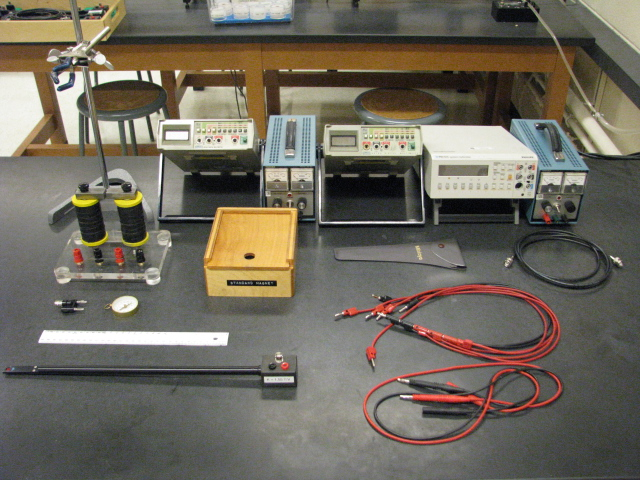
\includegraphics{/usr/local/master/labs/physics397-FA2017/0096-PHYS397FA2017/Hall-Effect-and-Magnetic-Hysteresis-Setup.jpg}
  \caption{Equipment Setup}
  \label{pic:HMSetup}
\end{figure}
Set up bench as shown in Figure \ref{pic:HMSetup}.


\section{Maintenance}
\begin{enumerate}
\item 
\item 
\end{enumerate}


\section{Critical Points of Failure}
There are currently no known critical points of failure.


\section{Notes to the Instructor}
\begin{enumerate}
\item Iron should be demagnetized before beginning experiment.
\item 
\item 
\end{enumerate}


\section{Prelab Questions}
\begin{enumerate}
\item Definitions:
  \begin{enumerate}
  \item Transducer: A device that converts one form of energy to another (example: a sensor converts pressure to an electrical signal)
  \item Hall Voltage: The voltage difference across an electrical conductor transverse to an electric current in the conductor and a magnetic field perpendicular to the current.
  \item Drift Velocity: The average velocity a particle attains due to an electric field.
  \item Charge Carrier Density: Number of charge carriers per unit volume.
  \item Electron Hole: The opposite of an electron but NOT a positron, rather the lack of an electron.
  \item Magnetic Moment: A quantity used to determine toque due to an external magnetic field.
  \item Hysteresis: The dependence on the output of a system not only on its current input but also on its history of past inputs.
  \end{enumerate}
\item Physical processes that exhibit hysteresis:
  \begin{enumerate}
  \item Engineering: Control systems, electronic circuits, user interface design
  \item Mechanics: elastic hysteresis (i.e. material internal friction in a rubber band), contact angle hysteresis, adsorption hysteresis, matric potential hysteresis
  \item Materials: magnetic hysteresis, electrical hysteresis, liquid-solid phase transitions
  \item Biology: cell biology and genetics, immunology, neuroscience (neurons that are unable to return to basal after a stimulus has been removed), respiratory physiology
  \item Economics: permanently higher unemployment, game theory and capital controls
  \end{enumerate}
\item Magnetic field strength can be found by rearranging Equation 13 from the lab manual to get,
$$
B=\frac{nqTV_H}{I}
$$
which results in a magnetic field strength of 1.7 mT.
\\
\\
\textit{Notes: Prelab sample answers were taken from Wikipedia.}
\end{enumerate}

\section{Data Requirements}
\begin{enumerate}[resume]
\item The magnitude of the Hall voltage resultant of the standard magnet was found to be 0.0651 $\pm$ 0.0002 V. From this, the numerical value of the proportionality constant, K was found to be 1.50 $\pm$ 0.07 T/V. The error was propagated using the following equation,
$$
u(K)=\sqrt{\left| \frac{\partial K}{\partial B}   \right|^2u(B)^2+\left| \frac{\partial K}{\partial V_H}  \right|^2u(V_H)^2}
$$
\item Hall Voltage vs. Electromagnetic Current at a constant control current of I$_C$=150.53 mA shown in Table 1.
  \begin{table}[h]
    \center
    \begin{tabular}{|c|c|c|c|c|c|c|c|c|c|c|c|}
      \hline
      A & $\delta$A & V & $\delta$V & A & $\delta$A & V & $\delta$V\\
      \hline
      0.000&0.01&0.001&0.0001&-0.929&0.01&-0.159&-0.0001\\
      0.091&0.01&0.012&0.0001&-0.998&0.01&-0.167&-0.0001\\
      0.199&0.01&0.031&0.0001&-1.093&0.01&-0.177&-0.0001\\
      0.304&0.01&0.054&0.0002&-1.204&0.01&-0.186&-0.0001\\
      0.426&0.01&0.079&0.0002&-1.298&0.01&-0.193&0.0001\\
      0.498&0.01&0.092&0.0002&-1.405&0.01&-0.200&0.0001\\
      0.606&0.01&0.111&0.0002&-1.499&0.01&-0.206&0.0001\\
      0.711&0.01&0.127&0.0002&-1.589&0.01&-0.211&0.0001\\
      0.795&0.01&0.139&0.0002&-1.642&0.01&-0.213&0.0001\\
      0.897&0.01&0.153&0.0003&-1.578&0.01&-0.212&0.0001\\
      0.997&0.01&0.165&0.0003&-1.491&0.01&-0.209&0.0001\\
      1.097&0.01&0.175&0.0003&-1.391&0.01&-0.204&0.0001\\
      1.203&0.01&0.184&0.0003&-1.291&0.01&-0.199&0.0001\\
      1.311&0.01&0.192&0.0003&-1.194&0.01&-0.193&0.0001\\
      1.403&0.01&0.198&0.0003&-1.099&0.01&-0.186&0.0001\\
      1.504&0.01&0.204&0.0003&-0.993&0.01&-0.178&0.0001\\
      1.599&0.01&0.209&0.0003&-0.894&0.01&-0.168&0.0001\\
      1.679&0.02&0.213&0.0003&-0.802&0.01&-0.159&0.0001\\
      1.576&0.01&0.210&0.0003&-0.696&0.01&-0.146&0.00005\\
      1.499&0.01&0.207&0.0003&-0.594&0.01&-0.132&0.00003\\
      1.399&0.01&0.203&0.0003&-0.505&0.01&-0.119&0.00002\\
      1.282&0.01&0.197&0.0003&-0.392&0.01&-0.100&0.000001\\
      1.190&0.01&0.191&0.0003&-0.303&0.01&-0.084&0.00002\\
      1.090&0.01&0.184&0.0003&-0.201&0.01&-0.064&0.00004\\
      0.990&0.01&0.176&0.0003&-0.087&0.01&-0.038&0.0001\\
      0.899&0.01&0.167&0.0003&0.000&0.01&-0.017&0.0001\\
      0.796&0.01&0.156&0.0003&0.096&0.01&0.007&0.0001\\
      0.693&0.01&0.144&0.0002&0.198&0.01&0.030&0.0001\\
      0.598&0.01&0.131&0.0002&0.299&0.01&0.052&0.0002\\
      0.496&0.01&0.116&0.0002&0.399&0.01&0.073&0.0002\\
      0.391&0.01&0.098&0.0002&0.495&0.01&0.091&0.0002\\
      0.290&0.01&0.080&0.0002&0.595&0.01&0.108&0.0002\\
      0.187&0.01&0.059&0.0002&0.697&0.01&0.124&0.0002\\
      0.108&0.01&0.041&0.0001&0.794&0.01&0.138&0.0002\\
      0.000&0.01&0.015&0.0001&0.899&0.01&0.151&0.0003\\
      -0.089&0.01&-0.008&0.0001&0.998&0.01&0.162&0.0003\\
      -0.199&0.01&-0.033&0.0001&1.103&0.01&0.172&0.0003\\
      -0.298&0.01&-0.055&0.00005&1.230&0.01&0.183&0.0003\\
      -0.396&0.01&-0.075&0.00003&1.299&0.01&0.188&0.0003\\
      -0.500&0.01&-0.095&0.00001&1.391&0.01&0.194&0.0003\\
      -0.595&0.01&-0.112&-0.00001&1.491&0.01&0.200&0.0003\\
      -0.704&0.01&-0.129&-0.00003&1.604&0.01&0.206&0.0003\\
      -0.809&0.01&-0.143&-0.00004&&&&\\
      \hline
    \end{tabular}
    \label{tbl:HMTable1}
    \caption{Hall voltage vs. Electromagnetic Current}
  \end{table}

\item Hall voltage vs. control current from 0 to 150 mA shown in Table 2.
  \begin{table}[h]
    \center
    \begin{tabular}{|c|c|c|c|}
      \hline
      Current (mA) & Error ($\delta$ mA) & Voltage (mV) & Error ($\delta$ mV)\\
      \hline
      14.3&0.1&13&0.0131\\
      23.4&0.2&22&0.0221\\
      50.3&0.3&46&0.0461\\
      69.7&0.3&64&0.0641\\
      77.8&0.3&71&0.0711\\
      92.8&0.4&85&0.0851\\
      103.1&0.4&94&0.0941\\
      115.4&0.4&105&0.1051\\
      132.0&0.5&120&0.1201\\
      139.3&0.5&126&0.1261\\
      149.6&0.5&133&0.1331\\
      \hline
    \end{tabular}
    \label{tbl:HMTable2}
    \caption{Hall voltage vs. Control Current}
  \end{table}
  
\item Sketch of Hall probe experimental system is shown in Figure \ref{fig:HMProbe}. The charge carriers are flowing with the current (the Hall voltage is positive and the direction of the magnetic field is pointing in the negative y-direction across the probe) which implies that the charge carriers are holes.
  \begin{figure}
    \center
    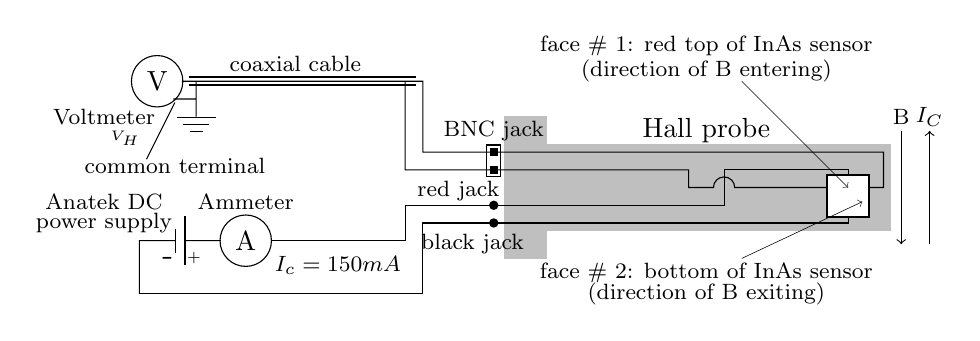
\begin{tikzpicture}[circuit ee IEC,scale=.9,inner sep=3pt]
      \draw[black,fill=lightgray,draw=lightgray](5.15,.5)rectangle(5.75,2.5); %grey for probe
      \draw[black,fill=lightgray,draw=lightgray](5.15,.9)rectangle(10.6,2.1); %grey for probe
      \draw(0,0)--(4,0)--(4,1)--(10,1)--(10,1.75)--(8.25,1.75)--(8.25,1.25)--(3.75,1.25)
      --(3.75,.75)--(1.5,.75)node[black,shape=circle,draw=black,fill=white]{A};
      \draw(1.15,.75) to [battery](0,.75)--(0,0); %bottom circuit
      \node[black,fill=white,draw=black,shape=circle,scale=1] at (.25,3){V}; %voltmeter
      \draw[double distance=2,thick](3.9,3)--(.7,3); %coaxial
      \draw(.6,3)--(3.75,3)--(3.75,1.75)--(7.75,1.75)--(7.75,1.5)--(8.1,1.5) arc (180:0:.15)
      --(10.5,1.5)--(10.5,2)--(4,2)--(4,3)--(4,3)--(.8,3)--(.8,2.5)--(.8,2.75)--(.48,2.75); %top circuit
      \draw(.8,2.5) to[ground](.8,2.28); %ground
      \node[black,fill=black,shape=circle,scale=.4] at(5,1){}; %black jack
      \node[black,fill=black,shape=circle,scale=.4] at(5,1.25){}; %red jack
      \draw(4.9,1.65)rectangle(5.1,2.1); %BNC jack
      \node[black,fill=black,shape=rectangle,scale=.5] at(5,2){}; %BNC jack
      \node[black,fill=black,shape=rectangle,scale=.5] at(5,1.75){}; %BNC jack
      \node[black,thick,fill=white,draw=black,shape=rectangle,scale=2.5] at(10,1.38){}; %InAs sensor
      %labels
      \node[font=\tiny] at (.77,.5){+};
      \node[font=\large] at (.4,.5){-};
      \node[font=\footnotesize] at (-.5,2.5){Voltmeter};
      \node[font=\tiny] at (-.2,2.2){$V_H$};
      \node[font=\footnotesize] at (.5,1.8){common terminal};
      \draw[thin](.1,1.9)--(.5,2.7);
      \node[font=\footnotesize] at (1.5,1.3){Ammeter};
      \node[font=\footnotesize] at (-.5,1.3){Anatek DC};
      \node[font=\footnotesize] at (-.5,1){power supply};
      \node[font=\footnotesize] at (2.2,3.25){coaxial cable};
      \node[font=\footnotesize] at (5,2.3){BNC jack};
      \node[font=\footnotesize] at (4.5,1.45){red jack};
      \node[font=\footnotesize] at (4.7,.7){black jack};
      \node[font=\normalsize] at (8,2.3){Hall probe};
      %\node[font=\footnotesize] at (10,2.3){edge \#3};
      %\node[font=\footnotesize] at (10,.7){edge \#4};
      %\node[font=\footnotesize] at (10.9,1.3){edge \#5};
      %\node[font=\footnotesize] at (9,1.3){edge \#6};
      \node[font=\footnotesize] at (8,3.5){face \# 1: red top of InAs sensor};
      \node[font=\footnotesize] at (8,3.15){(direction of B entering)};
      \draw[very thin,->](8.5,3)--(10,1.5);
      \node[font=\footnotesize] at (8,.3){face \# 2: bottom of InAs sensor};
      \node[font=\footnotesize] at (8,0){(direction of B exiting)};
      \draw[very thin,->](8.5,.5)--(10.2,1.3);
      \node[font=\footnotesize] at (2.8,.4){$I_c=150mA$};
      \node[font=\footnotesize] at (10.75,2.5){B};
      \draw[->] (10.75,2.3)--(10.75,0.7);
      \node[font=\footnotesize] at (11.15,2.5){$I_C$};
      \draw[<-] (11.15,2.3)--(11.15,0.7);
    \end{tikzpicture}
    \caption{Schematic of the Hall probe sensor setup.}
    \label{fig:HMProbe}
  \end{figure}
\end{enumerate}


\section{Calculations}

\begin{enumerate}[resume]
\item Drift velocity was calculated to be 
$$
V_D=\frac{1}{Kw}=(328\pm15)\ m/s
$$
using an experimental K value of (1.50$\pm$0.07) T/V and the given width of the Hall plate of (2.03$\pm$0.01) $\times 10^{-3}$ m from the lab manual. Multiplication/division error was propagated as mentioned in Data Requirement 4 of this companion guide.



\item Magnetic intensity vs. electromagnetic current shown in Table 3.
  \begin{table}
    \begin{tabular}{|c|c|c|c|c|c|c|c|c|c|c|c|}
      \hline
      A & $\delta$A & T & $\delta$T & A & $\delta$A & T & $\delta$T\\
      \hline
      0.000&0.01&8.15E+01&9E+00&-0.929&0.01&-1.30E+04&6E+02\\
      0.091&0.01&9.78E+02&5E+01&-0.998&0.01&-1.36E+04&6E+02\\
      0.199&0.01&2.53E+03&1E+02&-1.093&0.01&-1.44E+04&7E+02\\
      0.304&0.01&4.40E+03&2E+02&-1.204&0.01&-1.52E+04&7E+02\\
      0.426&0.01&6.44E+03&3E+02&-1.298&0.01&-1.57E+04&7E+02\\
      0.498&0.01&7.50E+03&4E+02&-1.405&0.01&-1.63E+04&8E+02\\
      0.606&0.01&9.05E+03&4E+02&-1.499&0.01&-1.68E+04&8E+02\\
      0.711&0.01&1.04E+04&5E+02&-1.589&0.01&-1.72E+04&8E+02\\
      0.795&0.01&1.13E+04&5E+02&-1.642&0.01&-1.74E+04&8E+02\\
      0.897&0.01&1.25E+04&6E+02&-1.578&0.01&-1.73E+04&8E+02\\
      0.997&0.01&1.35E+04&6E+02&-1.491&0.01&-1.70E+04&8E+02\\
      1.097&0.01&1.43E+04&7E+02&-1.391&0.01&-1.66E+04&8E+02\\
      1.203&0.01&1.50E+04&7E+02&-1.291&0.01&-1.62E+04&8E+02\\
      1.311&0.01&1.57E+04&7E+02&-1.194&0.01&-1.57E+04&7E+02\\
      1.403&0.01&1.61E+04&8E+02&-1.099&0.01&-1.52E+04&7E+02\\
      1.504&0.01&1.66E+04&8E+02&-0.993&0.01&-1.45E+04&7E+02\\
      1.599&0.01&1.70E+04&8E+02&-0.894&0.01&-1.37E+04&6E+02\\
      1.679&0.02&1.74E+04&8E+02&-0.802&0.01&-1.30E+04&6E+02\\
      1.576&0.01&1.71E+04&8E+02&-0.696&0.01&-1.19E+04&6E+02\\
      1.499&0.01&1.69E+04&8E+02&-0.594&0.01&-1.08E+04&5E+02\\
      1.399&0.01&1.66E+04&8E+02&-0.505&0.01&-9.70E+03&5E+02\\
      1.282&0.01&1.61E+04&8E+02&-0.392&0.01&-8.15E+03&4E+02\\
      1.190&0.01&1.56E+04&7E+02&-0.303&0.01&-6.85E+03&3E+02\\
      1.090&0.01&1.50E+04&7E+02&-0.201&0.01&-5.22E+03&2E+02\\
      0.990&0.01&1.44E+04&7E+02&-0.087&0.01&-3.10E+03&1E+02\\
      0.899&0.01&1.36E+04&6E+02&0.000&0.01&-1.39E+03&7E+01\\
      0.796&0.01&1.27E+04&6E+02&0.096&0.01&5.71E+02&3E+01\\
      0.693&0.01&1.17E+04&5E+02&0.198&0.01&2.45E+03&1E+02\\
      0.598&0.01&1.07E+04&5E+02&0.299&0.01&4.24E+03&2E+02\\
      0.496&0.01&9.46E+03&4E+02&0.399&0.01&5.95E+03&3E+02\\
      0.391&0.01&7.99E+03&4E+02&0.495&0.01&7.42E+03&3E+02\\
      0.290&0.01&6.52E+03&3E+02&0.595&0.01&8.81E+03&4E+02\\
      0.187&0.01&4.81E+03&2E+02&0.697&0.01&1.01E+04&5E+02\\
      0.108&0.01&3.34E+03&2E+02&0.794&0.01&1.13E+04&5E+02\\
      0.000&0.01&1.22E+03&6E+01&0.899&0.01&1.23E+04&6E+02\\
      -0.089&0.01&-6.52E+02&3E+01&0.998&0.01&1.32E+04&6E+02\\
      -0.199&0.01&-2.69E+03&1E+02&1.103&0.01&1.40E+04&7E+02\\
      -0.298&0.01&-4.48E+03&2E+02&1.230&0.01&1.49E+04&7E+02\\
      -0.396&0.01&-6.12E+03&3E+02&1.299&0.01&1.53E+04&7E+02\\
      -0.500&0.01&-7.75E+03&4E+02&1.391&0.01&1.58E+04&7E+02\\
      -0.595&0.01&-9.13E+03&4E+02&1.491&0.01&1.63E+04&8E+02\\
      -0.704&0.01&-1.05E+04&5E+02&1.604&0.01&1.68E+04&8E+02\\
      -0.809&0.01&-1.17E+04&5E+02&&&&\\
      \hline
    \end{tabular}
    \label{tbl:HMTable3}
    \caption{Magnetic Flux Density vs. Current}
  \end{table}



\item Graph of magnetic intensity vs. electromagnetic current is shown in Figure \ref{fig:HMGraph1}.
\begin{figure}[!ht]
\center
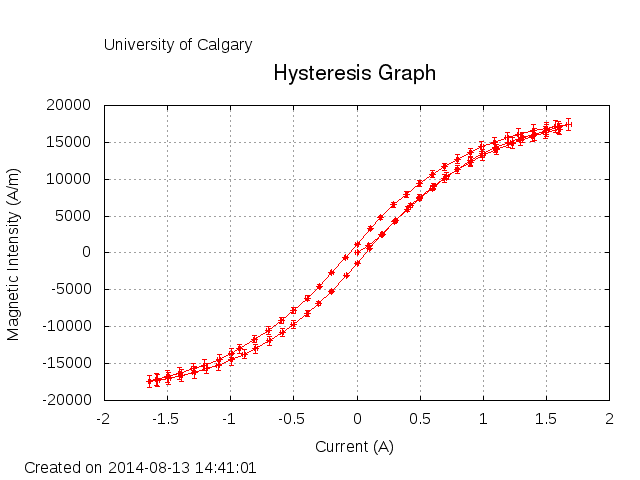
\includegraphics{/usr/local/master/labs/physics397-FA2017/0096-PHYS397FA2017/Hall-Effect-and-Magnetic-Hysteresis-Graph1.png}
\caption{Hysteresis Curve}
\label{fig:HMGraph1}
\end{figure}

\item Graph of Hall voltage vs. control current is shown in Figure \ref{fig:HMGraph2}.
\begin{figure}[!ht]
\center
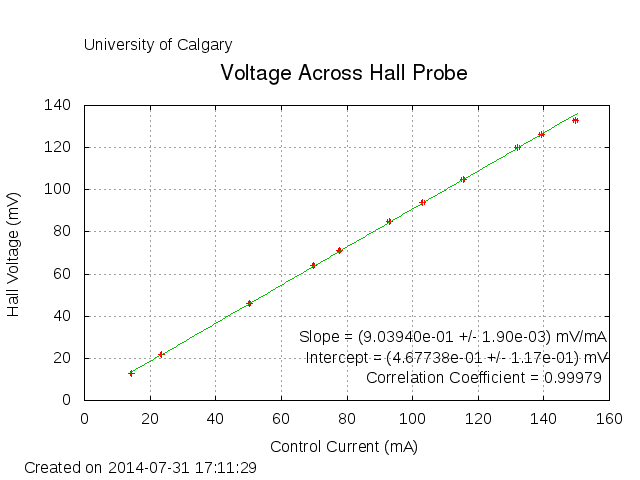
\includegraphics{/usr/local/master/labs/physics397-FA2017/0096-PHYS397FA2017/Hall-Effect-and-Magnetic-Hysteresis-Graph2.png}
\caption{Hall voltage vs. control current}
\label{fig:HMGraph2}
\end{figure}

\item The numerical value of the Hall coefficient, $R_H$, was found from the slope of Figure \ref{fig:HMGraph2} using the following equation,
$$
R_H=\frac{T}{B}\frac{V_H}{I}=\frac{T}{B}m = (7\pm1)\times10^{-4}
$$
where m is the slope from the graph. Multiplication/division error was propagated as mentioned in Data Requirement 4 of this companion guide.

\item The charge carrier density, n, for indium arsenside can be found using the following equation derived from Equation 13 of the lab manual,
$$
n=\frac{IB}{V_HqT}=\frac{1}{q}\frac{B}{mT}=\frac{1}{R_Hq}=(8\pm1)\times10^{21}\ m^{-3}
$$
where m is the slope of the Hall voltage vs. control current graph.
\end{enumerate}

\section{Discussion}

\begin{enumerate}[resume]
\item The graph of magnetic intensity vs. electromagnetic current represents a hysteresis curve. The plot generated in Figure \ref{fig:HMGraph2} shows how the Hall probe reacts to an increase in its control current. Since the Hall voltage increases with increasing control current it can be inferred that the magnetic field is also increasing. This happens because the iron is further magnetized by the current in the probe.
\item The remenance of this electromagnet is approximately 1000 A/m based on Figure \ref{fig:HMGraph1}.
\item The use of electromagnets is dependent on its ability to exhibit magnetic hysteresis. This occurs when the electromagnet is subjected to an external magnetic field where the magnetic force pushes charges of the opposite sign to each side. The charge carriers then stay in this state, which is known as hysteresis, and require an external magnetic field to be reapplied to change the orientation of the magnetization (or enough given time for the magnetization to diminish).
\item Two main sources of heat responsible for warming the Hall probe are the electromagnet and the current running within the Hall probe itself.
\item Applications for Hall probes are generally sensors such as a magnetometer. Applications for electromagnets are credit cards, hard disks, etc. since the memory is not easily erased.
\end{enumerate}

\AtEndDocument{\clearpage\ifodd\value{page}\else\null\clearpage\fi} % forces even page count, for double siding

\end{document}
